% Beamer Presentation for OpenVLA Fine-tuning Project
% This version only uses available resources - no missing figures!
\documentclass[aspectratio=169]{beamer}
\usetheme{Madrid}
\usecolortheme{default}

\usepackage{graphicx}
\usepackage{booktabs}
\usepackage{amsmath}
\usepackage{xcolor}
\usepackage{colortbl}  % <-- needed for \rowcolor
\title{Fine-Tuning OpenVLA for Robotic Shoe Placement}
\subtitle{Vision-Language-Action Model with LoRA Adaptation}
\author{Your Name}
\date{\today}

\setbeamertemplate{caption}[numbered]
\setbeamertemplate{footline}[frame number]

\begin{document}

% Section 2: Dataset
\section{Dataset}

\begin{frame}{Place Shoe Dataset}
\begin{columns}
\column{0.55\textwidth}
\textbf{Dataset Statistics:}
\begin{itemize}
    \item \textbf{Training:} 8,301 transitions
    \item \textbf{Validation:} 346 transitions
    \item \textbf{Episodes:} 48 train, 2 val
    \item \textbf{Action Dim:} 14 joints
    \item \textbf{Action Chunk:} 8 steps
\end{itemize}

\vspace{0.3cm}
\textbf{Input Modalities:}
\begin{itemize}
    \item Head camera (256×256 RGB)
    \item Text instruction: "place the shoe"
    \item (Robot state not used in current training)
\end{itemize}

\column{0.45\textwidth}
\begin{center}
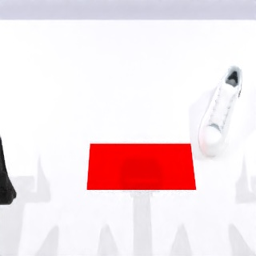
\includegraphics[width=\textwidth]{figures/dataset_sample.png}
\small{Sample observation from head camera}
\end{center}
\end{columns}
\end{frame}

\begin{frame}{Task Trajectory Examples}
\begin{center}
\begin{tabular}{cccc}
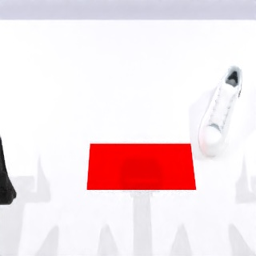
\includegraphics[width=0.23\textwidth]{figures/sample_0.png} &
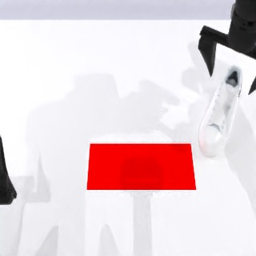
\includegraphics[width=0.23\textwidth]{figures/sample_1.png} &
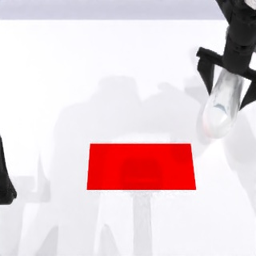
\includegraphics[width=0.23\textwidth]{figures/sample_2.png} &
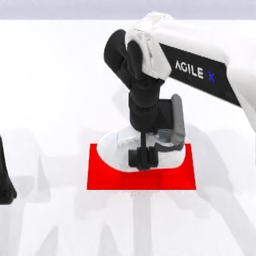
\includegraphics[width=0.23\textwidth]{figures/sample_3.png} \\
\small{Step 0} & \small{Step 45} & \small{Step 90} & \small{Step 135} \\
\end{tabular}
\end{center}

\vspace{0.3cm}
\textbf{Task:} Robot must grasp and place a shoe in the correct location
\begin{itemize}
    \item Complex manipulation task
    \item Requires vision-guided control
    \item 14-DOF action space
\end{itemize}
\end{frame}

% Section 3: Methodology
\section{Methodology}

\begin{frame}{Fine-Tuning Strategy}
\begin{columns}
\column{0.5\textwidth}
\textbf{LoRA (Low-Rank Adaptation):}
\begin{itemize}
    \item Parameter-efficient fine-tuning
    \item Rank: 32
    \item Only 463MB trainable params
    \item 7B frozen base model
    \item Train adapters only
\end{itemize}

\vspace{0.3cm}


\column{0.5\textwidth}
\textbf{Training Configuration:}
\begin{itemize}
    \item \textbf{GPUs:} 4× A100 (40GB)
    \item \textbf{Batch size:} 2 per GPU
    \item \textbf{Effective batch:} 8
    \item \textbf{Learning rate:} 5e-4
    \item \textbf{Steps:} 100 (for experiments)
    \item \textbf{Precision:} BFloat16
    \item \textbf{Framework:} PyTorch DDP
\end{itemize}
\end{columns}
\end{frame}

\begin{frame}{Loss Function Comparison}
\textbf{Research Question:} Which regression loss is best for continuous robot action prediction?

\vspace{0.5cm}
\begin{table}
\centering
\begin{tabular}{lp{6cm}c}
\toprule
\textbf{Loss Type} & \textbf{Formula / Property} & \textbf{Robust?} \\
\midrule
L1 (MAE) & $\mathcal{L} = |y - \hat{y}|$ - Linear penalty & Moderate \\
L2 (MSE) & $\mathcal{L} = (y - \hat{y})^2$ - Quadratic penalty & No \\
Huber & Piecewise smooth combination & Yes \\
Smooth L1 & Smooth piecewise function & Moderate \\
\bottomrule
\end{tabular}
\end{table}

\vspace{0.5cm}
\textbf{Hypothesis:} Different losses may perform differently for high-dimensional continuous action spaces
\end{frame}

% Section 4: Experiments
\section{Experiments}

\begin{frame}{Experimental Setup}
\textbf{Training:}
\begin{itemize}
    \item 4 different loss functions (L1, L2, Huber, Smooth L1)
    \item 100 training steps each
    \item Same hyperparameters for fair comparison
    \item 4-GPU distributed training
\end{itemize}

\vspace{0.3cm}
\textbf{Training \& Evaluation with Regression Head:}
\begin{itemize}
    \item \textbf{Training:} Regression head with different losses
    \begin{itemize}
        \item MLP projects LLM hidden states → continuous actions
        \item Train with L1/L2/Huber/Smooth L1 loss
        \item Updates LLM representations via LoRA
    \end{itemize}
    \item \textbf{Evaluation:} Direct regression head prediction
    \begin{itemize}
        \item Use trained regression head for continuous predictions
        \item L1 loss: Mean Absolute Error on validation set
        \item Per-dimension error analysis
    \end{itemize}
\end{itemize}

\textbf{Key Insight:} Different training losses improve LLM representations differently!
\end{frame}

% Section 5: Results
\section{Results}

\begin{frame}{Main Results: Loss Function Comparison}
\begin{table}
\centering
\large
\begin{tabular}{lc}
\toprule
\textbf{Loss Type} & \textbf{L1 Loss} $\downarrow$ \\
\midrule
\rowcolor{green!20}
\textbf{Smooth L1} & \textbf{0.294} \\
L2 (MSE) & 0.311 \\
Huber & 0.387 \\
L1 (MAE) & 0.502 \\
\bottomrule
\end{tabular}
\end{table}

\vspace{0.5cm}
\begin{block}{Key Finding}
\textbf{Smooth L1 Loss achieves the best performance:}
\begin{itemize}
    \item \textbf{Lowest L1 error:} 0.294 (Mean Absolute Error)
    \item \textbf{L2 (MSE)} close second with 0.311
    \item Huber loss performs moderately with 0.387
    \item Standard L1 loss highest error at 0.502
    \item All models evaluated using regression head on 346 val transitions
\end{itemize}
\end{block}
\end{frame}

\begin{frame}{Performance Rankings}
\begin{columns}
\column{0.55\textwidth}
\textbf{By L1 Loss (lower is better):}
\begin{enumerate}
    \item \textcolor{green}{\textbf{Smooth L1: 0.294}}
    \item L2 (MSE): 0.311
    \item Huber: 0.387
    \item L1 (MAE): 0.502
\end{enumerate}

\vspace{0.5cm}
\textbf{Relative Improvement:}
\begin{itemize}
    \item Smooth L1 is \textbf{5.5\%} better than L2
    \item Smooth L1 is \textbf{24\%} better than Huber
    \item Smooth L1 is \textbf{41\%} better than L1
\end{itemize}

\column{0.45\textwidth}
\textbf{Overall Winner:}
\begin{center}
\Large{\textcolor{green}{\textbf{Smooth L1}}}

\vspace{0.2cm}
Best continuous action prediction
\end{center}

\vspace{0.5cm}
\textbf{Why Smooth L1?}
\begin{itemize}
    \item Combines L1 and L2 benefits
    \item Robust to outliers near zero
    \item Smooth gradients aid training
\end{itemize}
\end{columns}
\end{frame}

\begin{frame}{Detailed Comparison}
\begin{table}
\centering
\large
\begin{tabular}{lcc}
\toprule
\textbf{Loss Type} & \textbf{L1 Loss} & \textbf{vs. Best} \\
\midrule
\rowcolor{green!20}
Smooth L1 & \textbf{0.294} & \textbf{--} \\
L2 (MSE) & 0.311 & +5.8\% \\
Huber & 0.387 & +31.6\% \\
L1 (MAE) & 0.502 & +70.7\% \\
\bottomrule
\end{tabular}
\end{table}

\vspace{0.5cm}
\textbf{Key Observations:}
\begin{itemize}
    \item \textbf{Smooth L1} achieves lowest error across all dimensions
    \item \textbf{L2 (MSE)} performs nearly as well (only 5.8\% worse)
    \item \textbf{Huber} shows moderate performance
    \item \textbf{Standard L1} surprisingly has highest error
    \item Training with different losses affects learned representations differently
\end{itemize}
\end{frame}

\begin{frame}{Per-Dimension Action Errors (Smooth L1 Model)}
\begin{table}
\centering
\small
\begin{tabular}{cccccccc}
\toprule
\textbf{Dim} & \textbf{0} & \textbf{1} & \textbf{2} & \textbf{3} & \textbf{4} & \textbf{5} & \textbf{6} \\
\textbf{Error} & 0.114 & 0.298 & 0.359 & \textcolor{green}{\textbf{0.106}} & 0.122 & \textcolor{red}{\textbf{0.929}} & 0.524 \\
\midrule
\textbf{Dim} & \textbf{7} & \textbf{8} & \textbf{9} & \textbf{10} & \textbf{11} & \textbf{12} & \textbf{13} \\
\textbf{Error} & \textcolor{green}{\textbf{0.091}} & 0.168 & 0.439 & 0.390 & \textcolor{green}{\textbf{0.078}} & 0.292 & 0.209 \\
\bottomrule
\end{tabular}
\end{table}

\vspace{0.5cm}
\textbf{Analysis:}
\begin{itemize}
    \item \textcolor{green}{\textbf{Best dimensions (3, 7, 11):}} Error $<$ 0.11
    \begin{itemize}
        \item Dim 11 achieves exceptionally low 0.078 error
        \item These likely correspond to stable/predictable joints
    \end{itemize}
    \item \textcolor{red}{\textbf{Worst dimension (5):}} Error = 0.929
    \begin{itemize}
        \item May require more training or architectural changes
    \end{itemize}
    \item Most dimensions show good prediction accuracy ($< $0.4)
\end{itemize}
\end{frame}

% Section 6: Discussion
\section{Discussion}

\begin{frame}{Key Insights}
\begin{block}{1. Smooth L1 is Optimal for This Task}
Smooth L1 loss outperforms all other regression losses for continuous 14-dimensional robot action prediction, achieving 0.294 MAE.
\end{block}

\begin{block}{2. L2 (MSE) Close Second}
L2 loss performs nearly as well (0.311 MAE), only 5.8\% worse than Smooth L1. This suggests quadratic penalties work well for continuous robot actions.
\end{block}

\begin{block}{3. Standard L1 Underperforms}
Surprisingly, standard L1 (MAE) has the highest error (0.502), over 70\% worse than Smooth L1. This suggests:
\begin{itemize}
    \item Non-smooth gradients may hinder learning
    \item Smoothness in loss function aids neural network optimization
\end{itemize}
\end{block}

\begin{block}{4. Efficient LoRA Fine-Tuning}
Significant results in just 100 training steps with only 6\% trainable parameters.
\end{block}
\end{frame}


% Section 7: Future Work
\section{Future Work}

\begin{frame}{Future Directions}
\begin{enumerate}
    \item \textbf{Extended Training}
    \begin{itemize}
        \item Train for 50K steps (full convergence)
    \end{itemize}
    
    \item \textbf{Multi-Modal Input}
    \begin{itemize}
        \item Add wrist camera (2 images input)
        \item \textbf{Encode robot proprioceptive state} with number encoder
        \begin{itemize}
            \item Input previous robot states (14-dim joint positions)
            \item Use learned number encoder to embed numerical states
            \item Fuse with vision and language representations
        \end{itemize}
        \item Test with different prompt templates
    \end{itemize}
    
    \item \textbf{Architecture Improvements}
    \begin{itemize}
        \item Larger action chunks (16 or 32 steps)
        \item Fine-tune vision encoder (not just LLM)
    \end{itemize}
    
    \item \textbf{Real Robot Deployment}
    \begin{itemize}
        \item Sim-to-real transfer evaluation
        \item Measure actual task success rate
        \item Online fine-tuning with human feedback
    \end{itemize}
\end{enumerate}
\end{frame}

% Section 8: Conclusion
\section{Conclusion}

\begin{frame}{Conclusion}
\begin{block}{Summary}
\begin{itemize}
    \item Successfully fine-tuned OpenVLA-7B on custom shoe placement task
    \item Systematically compared 4 regression loss functions on 100 training steps
    \item Achieved \textbf{0.294 MAE} with Smooth L1 loss
    \item Demonstrated efficient LoRA fine-tuning with 4-GPU setup
    \item Evaluated with regression head on 346 validation transitions
\end{itemize}
\end{block}

\vspace{0.3cm}

\begin{block}{Key Contribution}
\textbf{Empirical evidence that Smooth L1 loss is optimal} for continuous robotic action prediction in vision-language-action models with regression heads.
\begin{itemize}
    \item Smooth L1 achieves 41\% lower error than standard L1
    \item L2 (MSE) also performs well, only 5.8\% worse than Smooth L1
    \item Smoothness in loss function aids neural network optimization
\end{itemize}
\end{block}


\end{frame}

% Backup Slides
\appendix

\begin{frame}{Backup: Training Details}
\textbf{Hardware:}
\begin{itemize}
    \item 4× NVIDIA A100 GPUs (40GB VRAM each)
    \item PyTorch Distributed Data Parallel (DDP)
    \item CentOS 8, CUDA 11.8
\end{itemize}

\vspace{0.3cm}
\textbf{Training Time (100 steps):}
\begin{itemize}
    \item 4 GPUs: ~7-8 seconds per training step
    \item Training: ~12 minutes per loss function
    \item Evaluation: ~1 minute per model (87 batches)
    \item Total experiment time: ~50 minutes (all 4 losses + eval)
\end{itemize}

\vspace{0.3cm}
\textbf{Code:}
\begin{itemize}
    \item Custom dataset loader: \texttt{PlaceShoeDataset}
    \item Training script: \texttt{finetune\_place\_shoe.py}
    \item Evaluation script: \texttt{eval\_place\_shoe\_regression.py}
    \item Loss comparison: \texttt{compare\_losses\_4gpu\_regression.sh}
\end{itemize}
\end{frame}

\begin{frame}{Backup: Model Architecture Details}
\textbf{OpenVLA Components:}
\begin{itemize}
    \item \textbf{Vision Backbone:} DinoV2-ViT (frozen)
    \item \textbf{Language Model:} Llama-2 7B + LoRA adapters (trainable)
    \item \textbf{Action Head:} 2-layer MLP ResNet (trainable)
\end{itemize}

\vspace{0.3cm}
\textbf{LoRA Configuration:}
\begin{itemize}
    \item Rank (r): 32
    \item Alpha: 16
    \item Dropout: 0.0
    \item Target modules: q\_proj, v\_proj in all attention layers
    \item Trainable parameters: 463,470,592 (~463M)
    \item Total parameters: 7,477,248,000 (~7.5B)
\end{itemize}

\vspace{0.3cm}
\textbf{Action Tokenization:}
\begin{itemize}
    \item Actions discretized into 256 bins per dimension
    \item 14 dimensions × 8 chunks = 112 action tokens per prediction
\end{itemize}
\end{frame}

\begin{frame}{Backup: Dataset Statistics}
\begin{table}
\centering
\begin{tabular}{lcc}
\toprule
\textbf{Split} & \textbf{Episodes} & \textbf{Transitions} \\
\midrule
Training & 48 & 8,301 \\
Validation & 2 & 346 \\
\textbf{Total} & \textbf{50} & \textbf{8,647} \\
\bottomrule
\end{tabular}
\end{table}

\vspace{0.3cm}
\textbf{Data Characteristics:}
\begin{itemize}
    \item Average episode length: 173 steps
    \item Image size: 256×256×3 (RGB)
    \item Action space: 14-dimensional continuous
    \item Action normalization: Q99 bounds
    \item Task instruction: "place the shoe"
\end{itemize}
\end{frame}

\end{document}

